\documentclass[11pt,a4paper,twocolumn]{book}
\usepackage[utf8]{inputenc}
\usepackage{tikz}
\usetikzlibrary{er,positioning}
\usepackage[english]{babel}
\usepackage{amsmath}
\usepackage{amsfonts}
\usepackage{amssymb}
\usepackage{listings}
\usepackage{booktabs}
\usepackage{graphicx}
\author{Ege Özkan}
\title{CENG315 \\ \large{Information Managment Lecture Notes}}
\begin{document}
\lstset{language=SQL}
\newcommand{\missing}{\textit{(!*)}}
\newcommand{\unsure}{\textit{?*}}
\newcommand{\code}[1]{\texttt{#1}}
\newcommand{\join}{\ensuremath{\bowtie}}
\newcommand{\assign}{\ensuremath{\leftarrow}}
\maketitle
\chapter{Introduction - October 15, 2020}

\section{Databases and Database Systems}

Databases hold data. Database systems are software systems that manages the records in a database. There are five fundemental requirements for a database system.

\begin{itemize}
\item Database systems must be persistent, data must be storable and remain for the future.
\item Databases must be able to handle getting large.
\item Databases should be sharable, multiple users should be able to reach it at the same time.
\item Databases must be kept accurate.
\item Databases must be usable.
\end{itemize}

\subsection{Record Storage}

Databases can be made persistent in different ways.

\subsubsection{Storing database records in text files}

\begin{itemize}
\item Simplest approach.
\item One file per record type.
\item Each record could be a line of text, with its values seperated by tabs.
\end{itemize}

\begin{lstlisting}
1	joe	2020
2	amy	2013
3	lee	2000
\end{lstlisting}

Its advantages are the database system has to do very little, and a use could easily examine and modify the files with a text, but it is slow. \missing

\subsection{Data Models and Schema}

Data models are different ways to express connections between records while Schemas are the implementations of these methdos for a specific database.

\subsubsection{File-system v. Relational}

In the file system modal, each record type has a file, with one record per line, programs that read and write to the file is responsible for understanding this. In the relational data model, each record type has its \textbf{table} and each record has \textbf{fields} for each value. User access to the database happens via this record and field model and records that fit certain conditions can be quarried.\\

These models are at different levels of abstraction, relational model is a \textbf{conceptual model}, since there is no need to know \textbf{how} schemas are specified and implemented, the conceptual schema describes what the data \textit{is}. Whereas the file-system is called a \textbf{physical model}, physical schemas say how the data is \textit{implemented}.

\subsubsection{Physical Data Independence}

A conceptial schema is certainly nicer to use than a physical scheme. Operations on a conceptual schema is implemented by the database schema. Database system has a \textbf{database catalog} that contains descriptions of the physical and conceptual schemas. Givven an SQL querry, the database system translates the conceptual abstraction to the physical one and interract with it on the users behalf. If the user does not have to deal with the physical level, this is called the Physical Data Independence.

It is easy to use, quaries are optimized automatically and it is isolated from changes to the physical schema.

\subsubsection{Logical Data Independence}

The set of tables personalized for a particular user is called the user's \textbf{external schema}. If users can be given their own external schema in a database system, it is told that this Database System supports Logical Data Independence.\\

It has three benefits:

\begin{itemize}
\item Each users gets a customized external schema, they see only the information they need.
\item The user is isolated from changes to conceptual schema.
\item It is safer.
\end{itemize}

\section{Relational Databases}

The relational modal is a conceptual model since its schemas do not depend on the pyhsical level.

\subsection{Tables}

The database is organized into \textbf{tables}, which contain zero or more \textbf{records} (ie: table rows), and at least one \textbf{fields} (ie: the columns of the table.) Each record has a value for each field, and all fields has a specific \textbf{type}. Often, when discussing tables, the type information ignored.

\begin{figure}
\begin{lstlisting}
STUDENT(SId, SName, GradYear, MajorId)
DEPT(DId, DName)
COURSE(CId, Title, DeptID)
SECTION(SectId, CourseId, Prof, Year)
DEPARTMENT(DId, Name)
\end{lstlisting}
\caption{An example schema}
\label{schema:univesity}
\end{figure}

\subsubsection{Null Values}

A \texttt{null} value denotes a value that \textit{does not exist} or is \textit{unknown}. It occur if the data collection is incomplete or if data has not arrived yet.

\subsection{Superkeys and Keys}

In the relational model, the access to data is not handled by indices. Instead, a record must be referenced by specifying field values. Since not all values are guranteed to be unique for all users, a unique identifier field is called a \textbf{superkey} to distinguish it. Adding a field to a superkey, will generate another superket. A \textbf{key} is a superkey with the property that no subset of its fields is a super key.\\

\subsubsection{Primary Keys}

In the Schema at Figure \ref{schema:univesity}'s, \texttt{STUDENT} table \texttt{SId} is a key. Whereas in \texttt{SECTION} there may be multiple keys if each professor teaches only one class. Therefore, since a table may have multiple keys, a key is chosen as a \textbf{Primary Key}, whose  values \textit{should never be null}, and who is used to refeer to each record.\\

For instance, in Figure \ref{schema:univesity}, \texttt{STUDENT} table, \texttt{SId} can be the primary key. This is no coincidance, IDs are most times fit to be primary keys.

\subsubsection{Foreign Keys}

The information in a database is split among tables, these are not isolated from each other, a \textbf{foreign key} is a field (or fields) of one table which corresponds to the primary key of another table. For instance, in Schema at Figure \ref{schema:univesity}, \texttt{CourseId} of the \texttt{SECTION} table is a foreign key.\\

Foreign Keys can be used to create logical connections between different types of records. In the Schema at Figure \ref{schema:univesity}, \code{CourseId} of the \code{SECTION} table creates a logical connection between the \code{SECTION} table and \code{COURSE} table, since the objects these represent in real life, Sections and Courses are bound by a logical connection as well. (Each section is a section of a course).

\subsubsection{Foreign Keys and Referential Integrity}

The specification of a foreign key asserts \textbf{referential integrity}. Which requires each non-null foreign key value to be the key value of some record. Database system must ensure that if the primary keys of a table is modified in some ways, the foreign keys in other tables refeering to primary keys must also be updated accordingly, or set to \code{null} in worst case scenerio.

\subsection{Constraints}

A \textbf{constraint} describes the allowable states that fields can have in a table. There are four important kinds of constraints. \textbf{Null Value Constraints} limit fields to not have \code{null} values. \textbf{Key constraints} specify that two records cannot have the same value. \textbf{Referential integrity constraints} specify referential integrity, finally \textbf{integrity constraints}.

\subsubsection{Integrity constraints}

These constraints encodes \textit{business rules}. They can detect bad data entry and can enfore the \textit{rules} of the organization. They may apply to tables, individual records or the entire database.

\subsection{Tavle Specification in SQL}

\begin{lstlisting}[caption={the SQL specification of the STUDENT table},label={lst:student}]
create table STUDENT (
	SId int not null,
	SName varchar(10) not null,
	MajorId int,
	GradYear int,
	
	primary key (SId),
	foreign key (MajorId) references DEPT
		on update cascade
		on delete set null,
	check (SId > 0),
	check (GradYear >= 1863)
)
\end{lstlisting}

In Listing \ref{lst:student} we can see constraints and fields. The action specified with the \code{on delete} and \code{on update} keywords can be one of the following:

\begin{description}
\item[Cascade] causes the same query to apply to each foreign key record.
\item[Set null] causes the foreign key values to be set to null.
\item[Set default] causes the foreign key values to be set to their default value.
\item[No action] causes query to be rejectd if there exists and effected value with the foreign key.
\end{description}

\chapter{Relational Algebra - October 22, 2020}

\begin{table}[h]
    \centering
    \begin{tabular}{llll}
		ID & Name & Dept. Name & Salary\\
        \toprule
        22222 & Einstein & Physics & 95000\\
        12212 & Tesla & Physics & 4354\\
        \bottomrule
    \end{tabular}
    \caption{Instructors.}
    \label{tab:inst}
\end{table}

\section{Structure of Relational Databases}

Databases are structured with atrributes and values as tuples corresponding to those attributes.

\subsection{Attributes}
The domain of teh attribute is a set of allowed values. Attribute values are normally required to be \textbf{atomic}.

The \textbf{null} value is a special value that signifes that the value is unknown, or does not exist, it is a member of every domain. However, it causes complications.

\subsection{Schema vs Instance}

A database schema is the logical structure of the database. \texttt{instructor(ID, name, dept\_name, salary)}. A database instance is the snapshot of the database in a given time.

Using common attributes in relation schemas is one of \missing. There is also need for a \missing.

\subsection{Keys}

A \textbf{superkey} is a set of one or more attributes that allow us to identify uniquely a tuple in relation. Let $L \subset R$, superkey  $K$ is a \textbf{candidate key} if $K$ is minimal. One of the candidate keys is selected to be \textbf{primary key}, they should be chosen such that its attribute values are never or very rarely changed.\\

\textbf{Foreign key constraint} states that value in one relation must appear in another. \textbf{Referencing relation} is the relation that refeers to another and \textbf{Referenced relation} is the reference that is being referenced.

\section{Relational Query Languages}

A \textbf{query language} is a language in which a user requests infromation from the database. \textbf{Relational algebra} provides a set of operations that take one or more relations as input and return a relation as an output.

\section{Operations of Relational Algebra}

Relational algebra provides operations that take relations as input and returns relations as output.

\subsection{Select Operation}

Select operator selects $\sigma_p (r)$ (or \texttt{select(r, p)} to denote the selection of rows (horizontal selection) to denote selection on relation $r$ with respect to predicate $p$.\\

For instance, $\sigma_{A=B \land D>5}(r)$ would select tuples of relation $r$, such that its $A$ and $B$ attributes are equal and values of $D$ attribute is greater than 5\\

On the Table \ref{tab:inst}, $\sigma_{\text{dept\_name}=\text{"Physics"}(\text{instructor})}$ would return a tuple of instructors whose department is Physics.\\

Selection predicate can take comparasions using $=, \neq, >, \geq, <, \leq$ and multiple predicates can be combined using \textbf{connectives.} $\land, \lor$ and $\lnot$.\\

For instance on the department table with schema \texttt{department(dept\_name, building, budget)}, $\sigma_{\text{dept\_name}=\texttt{building}}(\text{department})$ would return departments whose names equal to their building's name.\\

\subsection{Project Operation}

An unary operation that returns its argument relation with certain attributes left out. $\Pi_{A_1, A_2, A_3, \dots, A_k}(r)$ or \texttt{project(r, {$A_1, A_2, A_3, \dots, A_k$})} where $A_n$ are attribute names and $r$ is a relation.\\

In essance project operation returns tuples with only the values whose attributes are listed in the operation.\\

\subsection{Composition of Relational Operations}

Since the result of a relational operation are itself a relations, operations can be given as input to other operations, ie: they can be composed together into a \textbf{relational-algebra expression}, finding the names ofa ll instructors in the physics department can be done by:

\begin{equation}
\Pi_{\texttt{name}}(\sigma_{\texttt{dept\_name} = \texttt{"Physics"}}(\texttt{instructor}))
\end{equation}

\subsection{Cartesian Product Operation}

Composes two relations together to a single product, $\texttt{instructor} \times \texttt{teaches}$ relation, where \texttt{instructor(id, name, dept\_name, salary)} and \texttt{teaches(id, course\_id, year} results in the relation \texttt{instructor$\times$teaches(instructor.id name, teaches.id, course\_id, year)}\\

However, as one can see, common attributes are not joined, therefore the cartessian product may not (and most likely will not) result in logical results.\\

When to attribute names are the same, they can be distinguished by attaching the name of the relation prior to the attribute name.\\

\subsection{Join Operation}

To avoid the mistake of illogical results, one can write:

\begin{equation}
\sigma_{\texttt{instructor.id}=\texttt{teaches.id}}(\texttt{instructor}\times\texttt{teaches}).
\end{equation}

The join operator is the equivalent of this expression. \textbf{Natural join} operation is denoted by $\join$ Outputs of the rows from the two input relations that have the same value on all atributes that have the same name is joined.\\

Consider relations $r$ and $s$, let $\theta$ be a predicate on attributes in the schema $r \cup s$. The join operation $r \join_\theta s$ is defined as $r \join_\theta s = \sigma_\theta (r \times s)$

Such as $\code{teaches} \join_{\code{teaches.id} = \code{instructor.id}}( \code{instructor})$ is equivalent to $\sigma_{\texttt{instructor.id}=\texttt{teaches.id}}(\texttt{instructor} \times \texttt{teaches})$

\subsection{Union Operation}

The union operation $r \cup s$ combines two relations as long as they have the same \textbf{arity} (number of attributes) and the attribute domains are compatible. (Same indexed attributes have the same domain.)\\

The expression $\pi_{\code{course\_id}}(\sigma_{\code{semester}=\code{"Fall"} \land \code{year} = 2017}(section) \cup \pi_{\code{course\_id}}(\sigma_{\code{semester} = \code{"Spring"} \land \code{year} = 2018}(section)$ on the relation \code{section} with schema \code{section(course\_id, sec\_id, semester, year, building, room, number, time\_slot\_id)} wil select \code{course\_id} row of the course that are though on Fall 2017 \textbf{or} Fall 2018.

\subsection{Set Intersection Operation}

Set intersection $s \cap r$ works exactly the same (and have the same assumptions.), but instead of working like \textit{or}, it works like \textbf{and}.

\subsection{Set Difference Operation} 

Set differnce $s - r$ works similar to intersection and union, but it selects those tuples that are on the first relation and \textbf{not} on the second relation.

\subsection{Rename Operation}

Given the relational algebra expression $E$, the expression $\rho_x(E)$ returns the expression $E$ under the name $X$.\\

It can also return an output whose attribute names are changed when they are listed $\rho_{x\{A_1, A_2, \dots, A_n\}}(r)$.

\subsection{Assignment Operation}

The assignment operation $\assign$ works like assignment in a programming language, relation algebra expressions can be assigned to temporary relation variables.

\begin{align*}
\code{Physics} \assign \sigma_{\code{dept\_name} = \code{"Physics"}}(\code{instructor})\\
\code{Musics} \assign \sigma_{\code{dept\_name} = \code{"Musics"}}(\code{instructor})\\
\code{Musics} \cup \code{Physics}
\end{align*}

\subsection{Equivalent Queries}

Since there is more than one way to write a query in relational algebra, queries that are not identical may be \textbf{equivalent}, they give the same result on any database.

\subsubsection{Alternative Notation}

On a related note, queries can be written with the alternative notation shown. For instance, \code{select(p, r)} instead of $\sigma_p (r)$

\chapter{Database Design - November 12, 2020}

\section{Design Phases}

\missing, First the database needs must be understood, after the database is designed conceptually. The final design is done in two phases, logical and phusical design, logical design is deciding on the schema, and phiscal design is choosing the implementation.

\section{Entity Relationship Model}
\scalebox{0.65}{
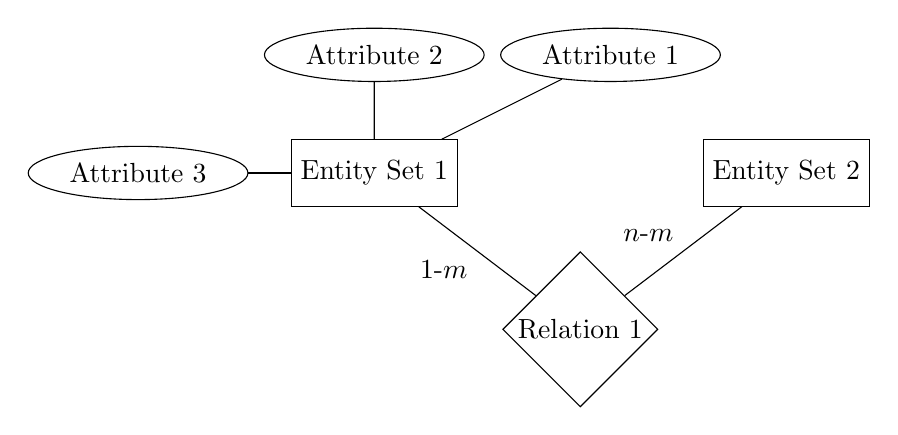
\begin{tikzpicture}[auto,node distance=1.5cm]
  % Create an entity with ID node1, label "Fancy Node 1".
  % Default for children (ie. attributes) is to be a tree "growing up"
  % and having a distance of 3cm.
  %
  % 2 of these attributes do so, the 3rd's positioning is overridden.
  \node[entity] (node1) {Entity Set 1}
    [grow=up,sibling distance=3cm]
    child {node[attribute] {Attribute 1}}
    child {node[attribute] {Attribute 2}}
    child[grow=left,level distance=3cm] {node[attribute] {Attribute 3}};
  % Now place a relation (ID=rel1)
  \node[relationship] (rel1) [below right = of node1] {Relation 1};
  % Now the 2nd entity (ID=rel2)
  \node[entity] (node2) [above right = of rel1]	{Entity Set 2};
  % Draw an edge between rel1 and node1; rel1 and node2
  \path (rel1) edge node {1-\(m\)} (node1)
    edge	 node {\(n\)-\(m\)}	(node2);
\end{tikzpicture}
}

Models and enterprise as a collection of \textbf{entities} and \textbf{relationships}. It is also called the ER diagram. It consists of three basic structures, \textbf{entity sets}, \textbf{relationship sets} and 

\begin{description}
\item[Entity] a thing or an object in the enterprise that is distinguishable from other objects, described by a set of \textit{attributes}.
\item[Relationship] An association among several entities.
\end{description}

Since entities are represented by a set of attributes, a subset of the attributes form a \textbf{primary key} of the entity set, uniquelly identifying each member of the sets.\\

Entity sets are represented in a similar fashion to UML class diagrams, with its attributes being the variables of the class. In the alternative notation, they are represented as rectangles, with its attributes (shown with elipses) tied to them. This alternative notation is shown in the picture at the start of subsection 3.2 (From https://texample.net/tikz/examples/er-diagram/)

\subsubsection{Complex Attributes}

Attributes can be grouped as simple and composite attributes, composite attributes can be divided into subparts. They may also be grouped as single-valued and multi-valued attributes, multivalued attributes may take more than one value at one time. Finally, a \textbf{derived} attribute is an attribute that can be derived from other attributes.\\

Composite attributes are shown as nested values in the UML-like notation. In the alternative notation, they are arguments bound to other arguments.

\subsubsection{Relationship Sets}

A relationship set is a mathametical relationship between two entity sets. Relationship sets are represented using diamonds between two entity sets. \textbf{Roles} are used to differ between two occurances of the same entity set in different rules, for instance, a course may be a prerequisette and the course name itself.\\

Relationship sets have \textbf{Degree}s, binary relationships involve two entity sets, which are most of them. But their degree may be higher.\\

\textbf{Cardinality} of a relationship refeers to the  number of entities connected in each entity set by a relationship,  a one-to-one relationship cocurs when the cardinality of a relationship is \textbf{contrainted} to at most one. The side(s) that is constrainted to at most one of themselves has a arrow head pointed at them in their connection to the relationship.\\

Cardinality constraints of relationships may be one-to-one, many-to-one, one-to-many or many-to-many.

The \textbf{Participation} is denoted with a double line or a single line, the \textbf{total participation}, indicated by a dobule line, means that every entity in the entity set participates in at least one relationship in the relationship setü while \textbf{partial participation} means that some entities may not participate in a relationship in the relationship set.\\

A line may have a text on it, of the form \textit{l..h}, where \textit{l} is the minimum and \textit{h} is the maximum cardinality. If an asterix (\textit{*}) is given for the maximum, that implies that there is no limit. A minimum value of 1 implies maximum cardinality.\\

In Ternary and above relationship sets, only one arrow is allowed to denote cardinality.

\subsubsection{Primary Key for Entity Sets}

By definition, individual entites are distinct, no entities in an entity set can have all their attributes the same, at least one attribute must differ, the primary key is the one attribute that distinguishes between all entities.

\subsubsection{Primary Key for Relationship Sets}

To distinguish among the various relationships of a relationship set, individual priamry keys of the entities in the relationship set denote the primary key for a relationship set is denoted by the union of primary keys of its entity sets.\\

The implication here is that, depending on the cardinality, for one-to-many relationships, the many side's keys are the minimal superkey and therefore , for many-to-many, the union of the keys take this role and for one-to-one, any one of the attributes may be chosen. \unsure \\

In conclusion, the idea is to chose the primary key from the side that repeats the least. The idea is \textit{how we can represent a connection using the least amount of keys?} We choose the many side, because, in one-to-many or many-to-one, because each many item will have \textbf{at most} one corresponding one item. On the other side, the choice literally does not matter for one-to-one, and on the other side of this, we have many-to-many where we need both sides to adequitelly identify a relationship, since everyone can have multiple onnections.

\subsubsection{Weak Entity Sets}

A weak entity is an entity that cannot be uniquely identified by its attributes alone.

\scalebox{0.65}{
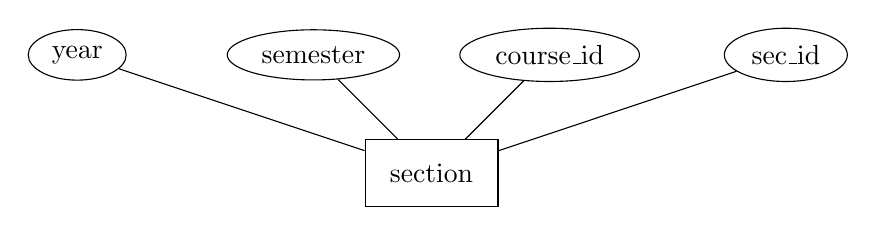
\begin{tikzpicture}[auto,node distance=1.5cm]
  % Create an entity with ID node1, label "Fancy Node 1".
  % Default for children (ie. attributes) is to be a tree "growing up"
  % and having a distance of 3cm.
  %
  % 2 of these attributes do so, the 3rd's positioning is overridden.
  \node[entity] (node1) {section}
    [grow=up,sibling distance=3cm]
    child {node[attribute] {\code{sec\_id}}}
    child {node[attribute] {\code{course\_id}}}
    child {node[attribute] {\code{semester}}}
    child {node[attribute]{\code{year}}};
\end{tikzpicture}
}

A \textbf{weak entity set} is one whose existence is dependent on another entity, called its \textbf{identifying entity}, the part of the primary key of this entity set is the primary key of the entity set it depends on as a \textbf{discriminator}. An entity set that is not a weak entity set is termed a \textbf{strong entity set}. Every weak entity must have a entity set it \textbf{existently depends} on.\\

In ER diagrams, a weak entity set is depicted via a double rectangle. Its discrimanotrs are underlined.\\

[Weak entity sets are simply entity sets that are dependant on other entity sets to exist.]

\section{Reducing ER Diagrams to Relational Schemas}

As a first approximation:

\begin{enumerate}
\item Turn each entity set into a relation with the same set of attributes.
\item Replace a relationship set by a relation whose attributes are the keys for the connected entity sets (and any descriptive attributes of the relationship sets).
\end{enumerate}

Weak entity sets change this somewhat.

\subsection{Representing entity sets}.

A strong entity set reduces to a schema with the same attributed, ie: A student entity set with attributes ID, name, and tot\_cred becomes \textit{student(\underline{ID}, name, tot\_cred)} A weak entity set becomes a table that includes a column for the rpimary key of the identifying strong entity set.\\

Composite Attributes are represented by dividing each composite part to normal attributes. [Composite attributes reduce to their subattributes.] Derived attributes are omitted completely.

Multivalued attributes map to brand new schemas, whose members are multiple values these attributes take. For instance, a student with a multivalued key phone number, maps to a phone number schema, whose members are all student's phone numbers, where a student may have multiple of them.\\


Many-to-one and one-to-many relationship sets that are total on the many-side can be represented by adding an extra attribute to the many side, containing the priamry of the one side. In one-to-one relationships, any side can be chosen as the many, albait, if the participation is not total, \code{NULL} values will occur.\\

Relations between weak entity sets and their corresponding strong entity sets are omitted as well, since they become redundant.

\subsection{Specialization}

Specialization is special entity set structure where a (weak) entity set is used as a subclass-like structure of another entity set. It can be overlapping (entity may occur in multiple specializations) or it may be disjoint, where this cannot occur.\\

Specializations are represented in schemas by creating a schema for the higher level entity, and then forming another schema for each lower-level entity set, include the primary key of the higher level entity set. Another method is to form a sechema for each entity set and include all local and inherited values. The drawback in the first is more queries being spent to look for a single entities records, and the for the second method more space being taken redunantly.\\

\subsubsection{Completeness Constraint}

Completeness constraint state wheter or not each entity in the higher level set must belong to a lower level entity set. Total Completeness means that it must, and Partial means it is not a must. The partial generalization is the default, when denoting a total generalization, a dashed line is drawn from the arrow, and on it the word \textit{total} is written.

\section{Design Problems}

There are certain design problems that may occur while designing a database system.

\subsubsection{Entities vs Attributes}

Certain attributes may be converted to entities on their own right if one wishes to store additional information about a specific attribute.

\subsubsection{Entities vs Relationship}

A guidline in deciding wheter or not something is an entity or a relationship is by asking if it is an \textit{actions}. Actions that occur between two of entities are relationships. Arguments directly related to relationships must become relationship attributes.

\subsubsection{Redunantant Atttributes}

Avoid repeating information. ER Diagrams \textit{are not} schemas, foreign keys are not needed to be shown if there is a relationship between them instead.

\end{document}
